\section[Caractère galiléen de certains référentiels]{Caractère galiléen approché de quelques référentiels courants}

    \subsection{Référentiel géocentrique et marée océanique}

        On se place dans $\mathcal{R}_{G}$ en translation (environ) circulaire par rapport à $\mathcal{R}_{C}$, voir la Figure~\ref{fig:refentiel_geocentrique_copernic}. On considère le mouvement d'un point matériel $M$ de masse $m$ au voisinage de la surface de la Terre par rapport à $\mathcal{R}_{G}$. Alors 
        \begin{equation*}
            m\vec{a}(M)_{/\mathcal{R}_{G}}=\vec{f}+m\vec{g}_{T}(M)+\sum_{\neq i}m\vec{g_i}(M)-m\vec{a}(T)_{/\mathcal{R}_C},
        \end{equation*}
        où $\vec{f}$ représentent les forces de contact (par exemple la pression), $\vec{g}_{T}$ est le champ de pesanteur dû à la Terre, $\vec{g_i}$ représente le champ de gravitation dû à un autre astre du système solaire, et $m\vec{a}_{T/\mathcal{R}_{C}}$ est simplement la force d'entraînement $\vec{F}_{e}$.

        En appliquant le principe fondamental de la dynamique à la terre par rapport à $\mathcal{R}_{C}$, on obtient 
        \begin{equation*}
            M_{T}\vec{a}(T)_{/\mathcal{R}_{C}}=\vec{R}^{\text{ext}}=\sum_{\neq i}M_T\vec{g_i}(T),
        \end{equation*}
        où l'on a fait l'hypothèse que la Terre était sphérique pour la dernière égalité. Ainsi, on a 
        \begin{equation*}
            \vec{a}(T)_{/\mathcal{R}_C}=\sum_{\neq i}\vec{g_i}(T).
        \end{equation*}
        Alors 
        \begin{equation*}
            \boxed{m\vec{a}(M)=\vec{f}+m\vec{g}_{T}(M)+m\left(\sum_{\neq i}\vec{g_i}(M)-\vec{g_i}(T)\right).}
        \end{equation*}

        \begin{definition}[Champ de marée]
            L'expression
            \begin{equation*}
                \vec{C}(M)\coloneqq\left(\sum_{\neq i}\vec{g_i}(M)-\vec{g_i}(T)\right),
            \end{equation*}
            définit le \textit{champ de marée}. C'est un terme différentiel.
        \end{definition}

        Notamment, le champ de marée dû à la Lune uniquement est
        \begin{equation*}
            \vec{C}_L(M)=\vec{g_L}(M)-\vec{g_L}(T).
        \end{equation*}

        \paragraph{Ordre de grandeur de $\left\lVert\vec{C_i}\right\rVert_{\text{max}}$.} 
            On a 
            \begin{equation*}
                \left\lVert \vec{C_i}\right\rVert=\calG M_i\left\lvert\frac{1}{(D_i-R_T)^{2}}-\frac{1}{D_i^{2}}\right\rvert.
            \end{equation*}
            Si $D_i\gg R_T$, on a 
            \begin{equation*}
                \frac{1}{(D_i-R_T)^{2}}=\frac{1}{D_i^{2}}\frac{1}{\left(1-\frac{R_T}{D_i}\right)^{2}}\sim\frac{1}{D_i^{2}}\left(1+\frac{2R_T}{D_i}\right).
            \end{equation*}
            Ainsi,
            \begin{equation*}
                \left\lVert \vec{C_i}\right\rVert_{\text{max}}=\calG M_i\frac{2R_T}{D_i^{3}}=\left\lVert\vec{g_i}(T)\right\rVert\underbrace{\frac{2R_T}{D_i}}_{\ll1}\ll\left\lVert \vec{g_i}\right\rVert.
            \end{equation*}
            
            On donne dans la Table~\ref{tab:champ_maree_soleil_lune} les ordres de grandeur des champs de marées dus au Soleil et à la Lune. On voit donc que le champ de marée lunaire est environ deux fois supérieur au solaire.
            
            \begin{table}
                \centering
                \begin{tabular}{l|c|c|c|c}
                    \toprule
                    & M (kg) & $D_i$ & $\left\lVert \vec{g_i}\right\rVert$ & $\left\lVert\vec{C}\right\rVert$\\ \midrule
                    Soleil & $2.10^{30}$ & $1.10^{11}$ & $1.10^{-2}$ & $5.10^{-7}$\\ \midrule
                    Lune & $7.10^{22}$ & $4.10^{8}$ & $3.10^{-5}$ & $1.10^{-6}$\\ \bottomrule
                \end{tabular}    
                \caption{Champs de marées dus au Soleil et à la Lune.}
                \label{tab:champ_maree_soleil_lune}
            \end{table}
        
        \paragraph{Interprétation du phénomène des marées océaniques.}
            \subparagraph{Effet dominant de la Lune.}

                Comme la période de révolution de la Lune autour de la Terre (environ 27 jours) est beaucoup moins longue que la période de révolution de la Terre autour de ses pôles (environ 24h), il y a deux marées hautes et deux marées basses par jour. Il y a un décalage d'environ 50 minutes par jour dû à la rotation de la Lune par rapport à la Terre.
            
            \subparagraph{Rôle du Soleil.}

                Selon la position de la Lune par rapport à la Terre et au Soleil, les effets de marées peuvent être atténués ou renforcés, voir la Figure~\ref{fig:lune_soleil_maree}. Durant la nouvelle Lune et la pleine Lune, le Soleil renforce l'effet de la Lune, ce sont des marées de vives-eaux. Au contraire, lors du premier et du dernier quartier, il y a une compensant partielle de l'effet de la Lune par le Soleil. Ce sont les marées de mortes-eaux.

                \begin{figure}
                    \centering
                    \tikzsetnextfilename{lune_soleil_maree}
                    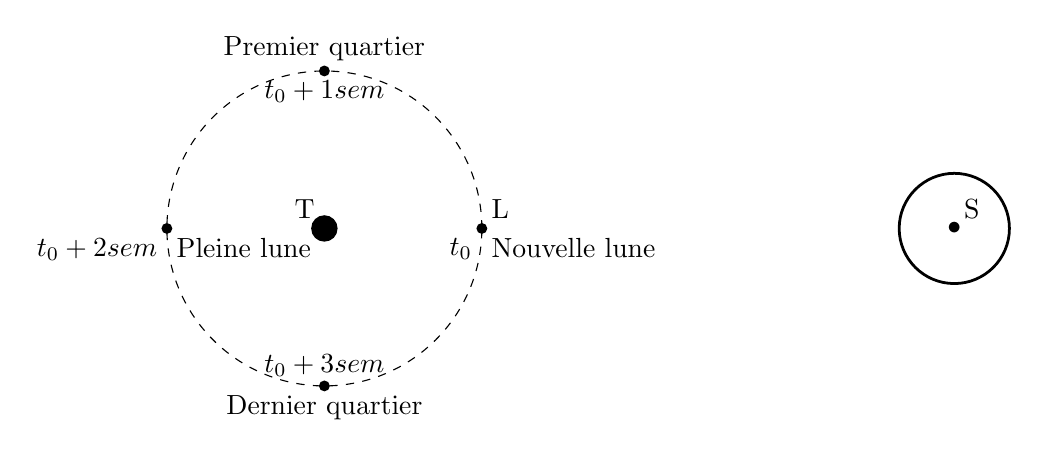
\begin{tikzpicture}[scale=1]  
                        % \helpgrid{3}{3}
                        \coordinate (T) at (0,0); \node at (T) [above left] {T};
                        \draw [line width=1pt,fill=black] (T) circle (0.15cm); 
                        \draw [dashed] (T) circle (2cm);
                        
                        \coordinate (S) at (8,0); \node at (S) [above right] {S}; \draw [line width=1pt] (S) circle (0.7cm);
                        \node at (S) {$\bullet$};

                        \coordinate (Lt) at (2,0); \node at (Lt) [above right] {L}; \node at (Lt) [below right] {Nouvelle lune}; \node at (Lt) [below left] {$t_0$};
                        \draw [line width=1pt,fill=black] (Lt) circle (0.05cm);

                        \coordinate (Ltt) at (0,2); \node at (Ltt) [above] {Premier quartier}; \node at (Ltt) [below] {$t_0+1\text{ sem}$};
                        \draw [line width=1pt,fill=black] (Ltt) circle (0.05cm);

                        \coordinate (Lttt) at (-2,0); \node at (Lttt) [below right] {Pleine lune}; \node at (Lttt) [below left] {$t_0+2\text{ sem}$};
                        \draw [line width=1pt,fill=black] (Lttt) circle (0.05cm);

                        \coordinate (Ltttt) at (0,-2); \node at (Ltttt) [below] {Dernier quartier}; \node at (Ltttt) [above] {$t_0+3\text{ sem}$};
                        \draw [line width=1pt,fill=black] (Ltttt) circle (0.05cm);
                    \end{tikzpicture}
                    \caption{Atténuation ou renforcement des effets de marées selon la position de la Lune par rapport à la Terre et au Soleil.}    
                    \label{fig:lune_soleil_maree}
                \end{figure}

    \subsection{Référentiel terrestre}
                
        On suppose le référentiel géocentrique $\mathcal{R}_{G}$ galiléen. On ne regarde que les effets de la rotation propre de la Terre.

        \subsubsection{Effets de la force centrifuge}

            On regarde de plus près la définition du poids. $\mathcal{R}_{T}$ est en rotation par rapport à $\mathcal{R}_{G}$ à une rotation angulaire
            \begin{equation*}
                \omega=\frac{2\pi}{T_{T}}=\frac{2\pi}{24\times3600}\approx 7.3.10^{-5}\text{rad}.s^{-1},
            \end{equation*}
            autour de l'axe $\vec{SN}$ fixe dans $\mathcal{R}_{G}$, voir la Figure~\ref{fig:rotation_terre_definition_poids}.

            \begin{figure}
                \centering
                \tikzsetnextfilename{rotation_terre_definition_poids}
                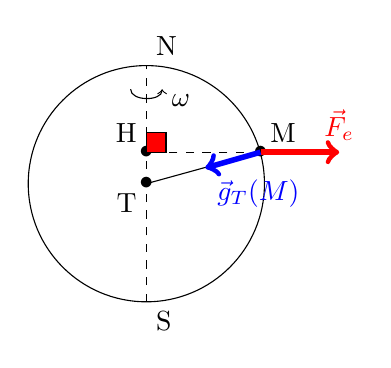
\begin{tikzpicture}[scale=1]  
                    % \helpgrid{3}{3}
                    \coordinate (T) at (0,0); \node at (T) [below left] {T};
                    \draw (T) circle (1.5cm); \node at (T) {$\bullet$};

                    \coordinate (S) at (0,-1.5); \node at (S) [below right] {S};
                    \coordinate (N) at (0,1.5); \node at (N) [above right] {N};
                    \draw [dashed] (S) -- (N);

                    \draw [->] (-0.2,1.2) to [bend right=90] (0.2,1.2);
                    \node at (0.2,0.85) [above right] {$\omega$};

                    \coordinate (M) at (1.45,0.4); \node at (M) [above right] {M}; \draw (T) -- (M); \node at (M) {$\bullet$};
                    \coordinate (H) at (0,0.4); \node at (H) [above left] {H}; \draw [dashed] (M) -- (H); \node at (H) {$\bullet$};
                    \draw [fill=red](H) rectangle ++(0.25,0.25);

                    \draw [red, ->, line width=2pt] (M) --++ (1,0) node [above] {$\vec{F}_e$};
                    \draw [blue, ->, line width=2pt] (M) --++ (-0.7,-0.2) node [below right] {$\vec{g}_T(M)$};
                \end{tikzpicture}
                \caption{Rotation de la Terre et définition du poids.}    
                \label{fig:rotation_terre_definition_poids}
            \end{figure}

            \paragraph{Équation du mouvement de M dans $\mathcal{R}_T$.}
            On a 
            \begin{equation*}
                m\vec{a}(M)_{/\mathcal{R}_T}=\vec{F}_e+m\vec{g_T}(M)+m\omega^{2}\vec{HM}-2m\vec{\omega}\wedge\vec{v}(M)_{/\mathcal{R}_T}.
            \end{equation*}

            \paragraph{Définition du poids/de la pesanteur.}
            Supposons qu'un fil à plomb soit en équilibre dans $\mathcal{R}_T$ et induise une tension (verticale) $\vec{T}$. Alors on a 
            \begin{equation*}
                \vec{0}=m\vec{g}_T+m\omega^{2}\vec{HM}+\vec{0}+\vec{T}.
            \end{equation*}
            Ainsi, $\vec{T}$, qui indique la verticale du lieu, est donné par
            \begin{equation*}
                \vec{T}=-m\left(g_T+\omega^{2}\vec{HM}\right).
            \end{equation*}

            \begin{definition}[Champ de pesanteur et champ de gravité]
                    En notant $\vec{g}$ le champ de pesanteur et $\vec{g}_{T}$ le champ de gravité, on a
                    \begin{equation*}
                        \boxed{
                        \vec{g}\coloneqq \vec{g}_T+\omega^{2}\vec{HM}.}
                    \end{equation*}
            \end{definition}

            $\vec{g}$ n'est donc pas tout à fait diriger vers $\vec{T}$. À l'équateur, $\omega^{2}R_t\approx0.03~m.s^{-2}$ avec $R_T\approx 6400~km$. En dynamique terrestre, $\vec{g}$ inclut la force centrifuge.

        \subsubsection{Effets qualitatifs de la force de Coriolis}

            Dans $\mathcal{R}_T$, on a 
            \begin{equation*}
                m\vec{a}(M)_{/\mathcal{R}_T}=\vec{f}+m\vec{g}-2m\vec{\omega}\wedge\vec{v}(M)_{/\mathcal{R}_T},
            \end{equation*}
            où $m\vec{g}$ représente le poids.

            \paragraph{Ordre de grandeur.}

                \subparagraph{Composante verticale de $\vec{F}_{\text{cor}}$.}

                    Elle est à comparer au poids. Elle vaut au maximum $2m\omega v$. Ainsi,
                    \begin{equation*}
                        \frac{\left\lVert\vec{F}_{\text{cor}}\right\rVert_{\text{max}}}{mg}=\frac{2\omega v}{g}\,\#\,\frac{14.10^{-5}}{10}\times v = 1,4.10^{-5}v.
                    \end{equation*}
                    Le plus souvent, la composante vertical est négligeable devant le poids. L'effet dominant est celui de la composante horizontale.

                \subparagraph{Échelles de temps.}

                    On compare le temps de l'expérience $T_{\text{exp}}$ au temps de révolution de la Terre $T_T$. On a 
                    \begin{equation*}
                        \frac{\left\lVert\vec{a}_{\text{cor}}\right\rVert}{\left\lVert\vec{a}(M)_{/\mathcal{R}T}\right\rVert}\,\#\,\frac{2\omega v}{v/T_{\text{exp}}}=2\omega T_{\text{exp}}=4\pi\frac{T_{\text{exp}}}{T_T}.
                    \end{equation*}
                    Le référentiel terrestre est quasi galiléen si $T_{\text{exp}}\ll 24h$.

                \subparagraph{Échelles de distance.}

                    On compare la longueur caractéristique présente dans l'expérience et $L_c$ (taille typique des déplacements dus à $\vec{F}_{\text{cor}}$). On a 
                    \begin{equation*}
                        \begin{aligned}
                            L_c & \approx a_{\text{cor}}\times T_{\text{exp}}^{2}=2\omega vT_{\text{exp}}^{2},\\
                            L_{\text{exp}} & \approx v\times T_{\text{exp}},
                        \end{aligned}
                    \end{equation*}
                    d'où 
                    \begin{equation*}
                        \frac{L_c}{L_{\text{exp}}}\,\#\,2\omega T_{\text{exp}}=4\pi\frac{T_{\text{exp}}}{T_T}.
                    \end{equation*}

            \paragraph{Expression de $\vec{F}_{\text{cor}}$ à la surface de la Terre.}

                On note $\lambda$ la latitude, voir la Figure~\ref{fig:expression_force_coriolis_surface_terre}. On note $(X,Y,Z)$ la base de projection (voir la Figure). On note 
                \begin{equation*}
                    \vec{v}(M)_{/\mathcal{R}_T}=\begin{pmatrix}
                        \dot{X}\\\dot{Y}\\\dot{Z}
                    \end{pmatrix}_{u_X,u_Y,u_Z}.
                \end{equation*}
                Alors
                \begin{equation*}
                    \vec{\omega}=\begin{pmatrix}
                        -\omega\cos\lambda\\0\\\omega\sin\lambda
                    \end{pmatrix},
                \end{equation*}
                d'où
                \begin{equation*}
                    \vec{\omega}\wedge\vec{v}=\begin{pmatrix}
                        -\omega\cos\lambda\\0\\omega\sin\lambda
                    \end{pmatrix}\wedge\begin{pmatrix}
                        \dot{X}\\\dot{Y}\\\dot{Z}
                    \end{pmatrix}=\begin{pmatrix}
                        -\omega\dot{Y}\sin\lambda\\
                        \omega\dot{X}\sin\lambda+\omega\dot{Z}\cos\lambda\\
                        -\omega\dot{Y}\cos\lambda
                    \end{pmatrix},
                \end{equation*}
                et
                \begin{equation*}
                    \vec{F}_{\text{cor}}=2m\omega\begin{pmatrix}
                        \omega\dot{Y}\sin\lambda\\
                        \omega\dot{X}\sin\lambda+\omega\dot{Z}\cos\lambda\\
                        -\omega\dot{Y}\cos\lambda
                    \end{pmatrix}.
                \end{equation*}

                \begin{figure}
                    \centering
                    \tikzsetnextfilename{expression_force_coriolis_surface_terre}
                    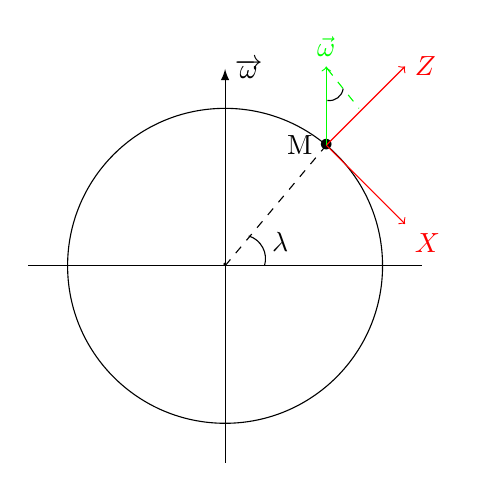
\begin{tikzpicture}[scale=1]
                        %\helpgrid{2}{2};
                        \coordinate (O) at (0,0);
                        \coordinate (M1) at (50:2cm);
                        \draw [color=black,smooth] (0,0) circle (2);
                        \draw (-2.5,0) --++ (5,0);
                        \draw [->,-latex] (0,-2.5) --++(0,5) node [right] {$\overrightarrow{\omega}$};
                        
                        \node at (O) {$\cdot$};
                        \node at (M1) {$\bullet$};
                        \node at (M1) [left=1.5] {M};
                        \draw [dashed] (O) -- (M1);
                        \draw [->, color=red] (M1) --++ (1, 1) node [right] {$Z$};
                        \draw [->, color=red] (M1) --++ (1, -1) node [below right] {$X$};
                        \draw [->, color=green] (M1) --++ (0, 1) node [above] {$\vec{\omega}$};
                        \draw [dashed, color=green] (1.3, 2.5) -- (1.7, 2);
                        \draw  (1.3,2.1) to [bend right=45] (1.5,2.25);
                        \draw  (0.5,0) to [bend right=45] (0.3,0.38);
                        \node at (0.7,0.3) {$\lambda$};
                    \end{tikzpicture}
                    \caption{Expression de la force de Coriolis à la surface de la Terre.}
                    \label{fig:expression_force_coriolis_surface_terre}
                \end{figure}

            \paragraph{Mouvements horizontaux : $\dot{Z}=0$.}

                On a 
                \begin{equation*}
                    \vec{F}_{cor,\text{horizontale}}=2m\omega\sin\lambda\begin{pmatrix}
                        \dot{Y}\\-\dot{X}\\0
                    \end{pmatrix}=-2m\omega\sin\lambda \vec{u}_Z\wedge\vec{v}.
                \end{equation*}
                Ainsi, dans l'hémisphère sud, on a $\lambda<0$ et $\vec{F}_{\text{cor}}$ est dans le même sens que $\vec{u_Z}\wedge\vec{v}$ : il y a une déviation vers la gauche. Dans l'hémisphère nord, on a $\lambda>0$ et on voit donc une déviation vers la droite.

                \subparagraph{Anticyclones et dépressions.}

                    La force de Coriolis justifie les mouvements des anticyclones et dépressions. On montre ce qu'il se passe dans l'hémisphère nord sur la Figure~\ref{fig:anticyclone_depression_hemisphere_nord}. En ordre de grandeur, on a $L_{\text{exp}}\approx 1000~km$ et $v\approx 10~m.s^{-1}$. Ainsi, $T_{\text{exp}}\,\#\,10^{5}~s$. Or $T_T=86400~s\,\#\,10^{5}~s$. Ainsi, $L_c\approx L_{\text{exp}}$.

                    \begin{figure}
                        \centering
                        \tikzsetnextfilename{anticyclone_depression_hemisphere_nord}
                        \begin{tikzpicture}[scale=1]
                            %\helpgrid{2}{2};
                            
                            \node at (0,2) {Anticyclone};
                            \draw[
                                decoration={markings, mark=at position 0.625 with {\arrow{<}}},
                                postaction={decorate}
                                ]
                                (0,0) circle (1);
                            \draw (0,0) circle (0.3); \node at (0,0) {$+$};

                            \draw (60:1.5cm) circle (0.3); \node at (60:1.5cm) {$-$};
                            \draw (0:1.5cm) circle (0.3); \node at (0:1.5cm) {$-$};
                            \draw (-60:1.5cm) circle (0.3); \node at (-60:1.5cm) {$-$};
                            \draw (120:1.5cm) circle (0.3); \node at (120:1.5cm) {$-$};
                            \draw (-120:1.5cm) circle (0.3); \node at (-120:1.5cm) {$-$};
                            \draw (180:1.5cm) circle (0.3); \node at (180:1.5cm) {$-$};

                            \node at (5,2) {Dépression};
                            \draw[
                                decoration={markings, mark=at position 0.625 with {\arrow{>}}},
                                postaction={decorate}
                                ]
                                (5,0) circle (1);
                            \draw (5,0) circle (0.3); \node at (5,0) {$-$};

                            \draw ($(5,0) + (60:1.5cm)$) circle (0.3); \node at ($(5,0) + (60:1.5cm)$) {$+$};
                            \draw ($(5,0) + (0:1.5cm)$) circle (0.3); \node at ($(5,0) + (0:1.5cm)$) {$+$};
                            \draw ($(5,0) + (-60:1.5cm)$) circle (0.3); \node at ($(5,0) + (-60:1.5cm)$) {$+$};
                            \draw ($(5,0) + (120:1.5cm)$) circle (0.3); \node at ($(5,0) + (120:1.5cm)$) {$+$};
                            \draw ($(5,0) + (-120:1.5cm)$) circle (0.3); \node at ($(5,0) + (-120:1.5cm)$) {$+$};
                            \draw ($(5,0) + (180:1.5cm)$) circle (0.3); \node at ($(5,0) + (180:1.5cm)$) {$+$};
                        \end{tikzpicture}
                        \caption{Sens des anticyclones et dépressions dans l'hémisphère nord.}
                        \label{fig:anticyclone_depression_hemisphere_nord}
                    \end{figure}

                \subparagraph{Tourbillons dans un lavabo.}

                    On a $L_{\text{exp}}\approx 10~cm$, $v\approx 10~cm.s^{-1}$, $T_{\text{exp}}\approx 1~s$, ainsi 
                    \begin{equation*}
                        L_{\text{cor}}\,\#\,L_{\text{exp}}\frac{T_{\text{exp}}}{T_T}=10^{-6}~m=1~\mu m.
                    \end{equation*}

                \subparagraph{Pendule de Foucault (1851).} Ce pendule dévie vers la droite. À l'équateur, on a $\lambda=0$ donc il n'y a pas de déviation. Au pôle nord, l'effet est maximum. Le plan d'oscillation tourne à $\omega$ par rapport à $\mathcal{R}_{G}$.
            
            \paragraph{Mouvement vertical de chute libre : déviation vers l'est. Expérience de Reich (1833).}

                On considère un puits de mine de profondeur $h=100~m$. Lorsqu'un objet tombe dans ce puits, on observe une légère déviation vers l'est (quelques millimètres). On reprend la Figure~\ref{fig:expression_force_coriolis_surface_terre} et on considère que $\left\lvert\dot{X}\right\rvert,\left\lvert\dot{Y}\right\rvert\ll\left\lvert\dot{Z}\right\rvert$. Alors 
                \begin{equation*}
                    \vec{F}_c=-2m\omega\dot{Z}\cos\lambda \vec{u_Y},
                \end{equation*}
                et $\dot{Z}<0$ donc $\vec{F}_c$ est dirigé vers l'est. En ordre de grandeur, on a 
                \begin{equation*}
                    L=\frac{1}{2}gt^{2},
                \end{equation*}
                donc 
                \begin{equation*}
                    T_{\text{exp}}=\sqrt{\frac{2h}{g}}\,\#\,\sqrt{\frac{h}{g}},
                \end{equation*}
                et ainsi
                \begin{equation*}
                    L_c\,\#\,\underbrace{L_{\text{exp}}}_{h}\times\frac{T_{\text{exp}}}{T_T}=\frac{h^{3/2}}{\sqrt{g}T_T}\,\#\,10^{-3}~m.
                \end{equation*}

                    

            
            

        